\chapter{Resultados y Discusiones}
% [En este capítulo se presentan los resultados obtenidos correspondientes al proyecto descrito en el capítulo anterior. Los resultados se pueden presentar en tablas o gráfica y deben ser redactados y organizados de tal manera que sea fácil de comprender por los lectores.

% La los resultados no se explican por si mismo, por lo que es necesario una discusión que los explique y muestre cómo ayudan a resolver el problema definido en el capítulo 1. La discusión puede mencionar someramente los resultados antes de discutirlos, pero no debe repetirlos en detalle. No prolongues la discusión citando trabajos ``relacionados'' o planteando explicaciones poco probables. Ambas acciones distraen al lector y lo alejan de la discusión realmente importante. La discusión puede incluir recomendaciones y sugerencias para investigaciones futuras, tales como métodos alternos que podrían dar mejores resultados, tareas que no se hicieron y que en retrospectiva debieron hacerse, y aspectos que merecen explorarse en las próximas investigaciones.]

% El proyecto finalizado, se compone de una cantidad aproximada de 3700 líneas de código, como se puede observar en el análisis de la herramienta \texttt{cloc} en la Figura \ref{fig:cloc}. Este proyecto se compone principalmente de componentes en Vue y scripts de Python.

% \begin{figure}[!ht]
%    \centering
%    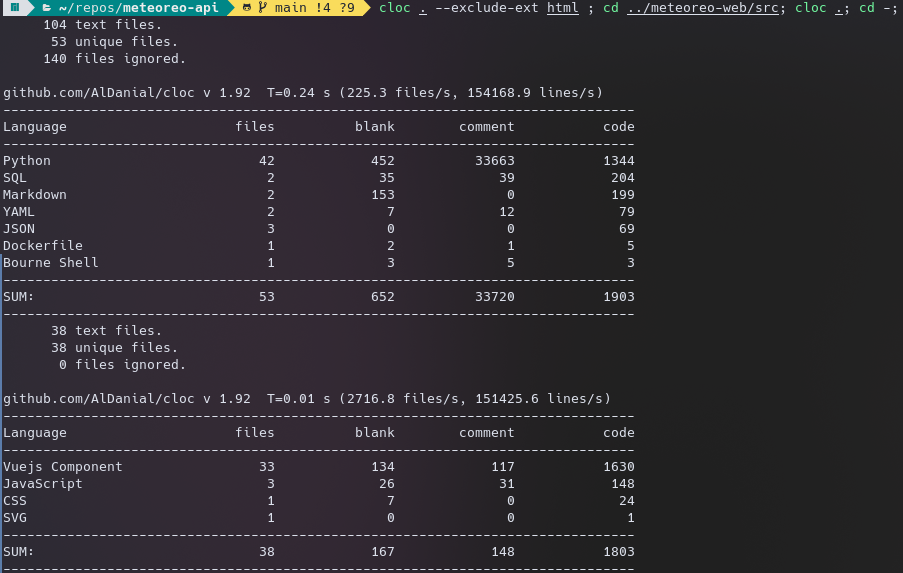
\includegraphics[width=0.8\linewidth]{images/screenshots/cloc}
%    \caption{Conteo de líneas de código.}
%    \label{fig:cloc}
% \end{figure}

Con la ayuda de la herramienta \href{https://locust.io/}{Locust}, se realizó una prueba de estrés y carga al sistema. Esta prueba se configuró para realizar pruebas en el sistema final en el que se realizó despliegue, la prueba se compone de dos rutas a probar (véase Listado \ref{lst:locust-config}), a las cuales se les realizarán peticiones con una cantidad creciente de usuarios concurrentes. Después de haber instalado la librería, se realizaron las pruebas con el comando \texttt{locust -H http://148.210.21.98:81 -u 50 -r 0.1 -t 300s --autostart}.

Al analisar la gráfica resultante, la Figura \ref{fig:locust-graphs}, de las pruebas, es posible observar que el tiempo de respuesta incrementa de forma lineal conforme a la cantidad de usuarios, comenzando con menos de 1 segundo por respuesta e incrementando hasta alcanzar casi 50 segundos por respuesta al tener a 50 usuarios concurrentes.

\begin{listing}
\begin{minted}[%
   breaklines
]{python3}
from locust import HttpUser, task

class API(HttpUser):
    @task
    def get_drivers(self):
        self.client.get("/api/v1/drivers/")

    @task
    def get_stations(self):
        self.client.get("/api/v1/stations/",  auth=("admin", "pass"))
\end{minted}
\caption{\texttt{lcoustfile.py} configuración de pruebas.}
\label{lst:locust-config}
\end{listing}


\begin{figure}[!ht]
   \centering
   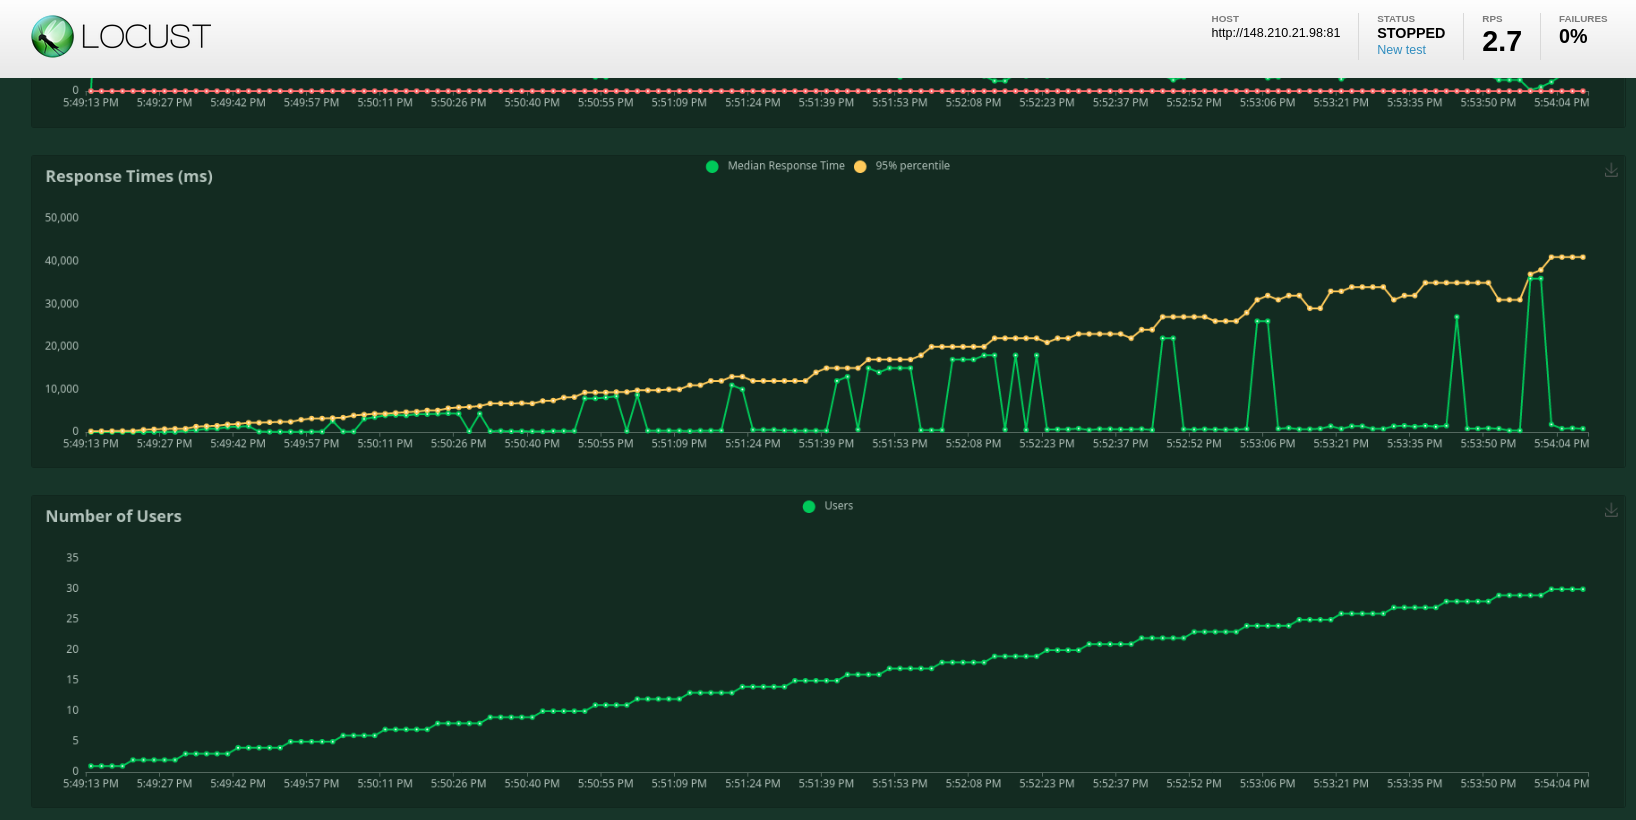
\includegraphics[width=1\linewidth]{images/screenshots/locust_graphs.png}
   \caption{Gráfica de usuarios y tiempos de respuesta creada con Locust.}
   \label{fig:locust-graphs}
\end{figure}

Sin embargo, al revisar el análisis de tiempo de respuesta por ruta presente en la Figura \ref{fig:locust-analysis}, es posible observar una diferencia significativa entre el tiempo de respuesta de la ruta \texttt{/api/v1/drivers}, con un máximo de 1.825s y la ruta \texttt{/api/v1/stations} con un máximo de 41.937s. Esto puede deberse a que la primer ruta mencionada no realiza tareas de lectura en la base de datos. Esto implicaría que la solución implementada para el almacenamiento de datos, una base de datos MariaDB en Docker en la misma máquina virtual que donde está alojado el API, no es una solución óptima para el problema.

\begin{figure}[!ht]
   \centering
   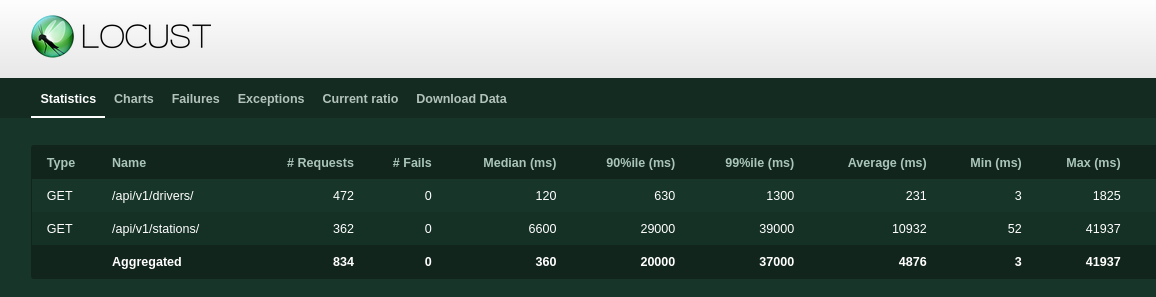
\includegraphics[width=1\linewidth]{images/screenshots/locust_analysis.png}
   \caption{Estadísticas de pruebas por ruta.}
   \label{fig:locust-analysis}
\end{figure}

